\documentclass[11pt]{article}
\usepackage[margin=1.25in]{geometry}
\usepackage{graphicx,booktabs,amsmath,tikz,caption,float}
\usepackage[hidelinks]{hyperref}
\captionsetup{font=small}

\title{Results from the Dual-Sided Readout of the BIC Test-Beam Stack\\[4pt]\large A repeat of the 2017 dual-sided EmCal study with run 3062}
\author{Tanner, Martin, Ravi, Claude}
\date{October 28, 2026}

\begin{document}
\maketitle

\section*{Setup}

In February 2017 a sPHENIX EmCal module with a SiPM at each end was tested at the Fermilab Test Beam Facility,
and the light sharing and the left--right timing were measured as a function of the beam position along the
module~\cite{note2017}. This note repeats that study with the barrel imaging calorimeter (BIC) test-beam stack,
using run 3062. The purpose, as in 2017, is
\begin{itemize}
  \item to measure the light sharing between the two ends with the shower at a known position along the fibres;
  \item to measure the time difference between the two ends as a function of that position;
  \item to judge how well a single shower can be placed along the fibres from either quantity.
\end{itemize}

The stack consists of five scintillating-fibre layers (SFIL1--5), each made of cells 19.05\,mm high with fibres
about 510\,mm long, read out at both ends (``North'' and ``South'') by summed SiPM boards. The SFIL1--4 signals
are digitised by HGCROC chips on the KCU0 readout: 20 ADC samples per trigger at 40\,MHz, i.e.\ one sample every
25\,ns. This is the main difference from 2017, where the waveforms were sampled by a DRS4 at 2\,GS/s (0.5\,ns).

The module was not moved during the run. Instead, the trigger is the OR of four scintillator paddles placed along
the fibre direction, and the paddle that fired tags the beam position for each event (Fig.~\ref{fig:setup}). An
AstroPix silicon layer in front of SFIL1 gives an independent, continuous position for a subset of showers.

We use the beam cell (cell~3) of SFIL2 and SFIL3:

\begin{center}
\begin{tabular}{llll}
\toprule
layer & cell & South channel & North channel \\
\midrule
SFIL2 & 3 & KCU0 29 & KCU0 173 \\
SFIL3 & 3 & KCU0 52 & KCU0 196 \\
\bottomrule
\end{tabular}
\end{center}

\begin{figure}[H]
\centering
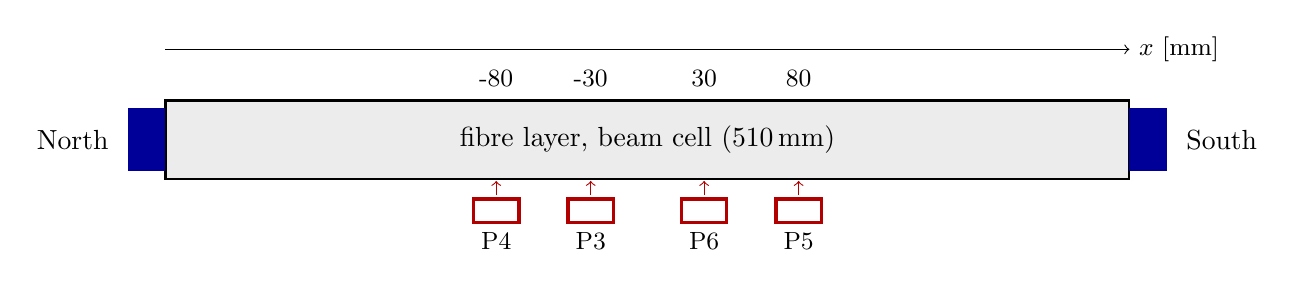
\begin{tikzpicture}[x=0.024cm,y=1cm]
  \fill[gray!15] (-255,0) rectangle (255,1.0);
  \draw[thick] (-255,0) rectangle (255,1.0);
  \node at (0,0.5) {fibre layer, beam cell (510\,mm)};
  \fill[blue!60!black] (-275,0.1) rectangle (-255,0.9); \node[anchor=east] at (-280,0.5) {North};
  \fill[blue!60!black] (255,0.1) rectangle (275,0.9);   \node[anchor=west] at (280,0.5) {South};
  \foreach \x/\p in {-80/P4,-30/P3,30/P6,80/P5} {
    \draw[red!70!black, very thick] (\x-12,-0.55) rectangle (\x+12,-0.25);
    \node[below] at (\x,-0.55) {\small \p};
    \node[above] at (\x,1.05) {\small \x};
    \draw[->, red!70!black] (\x,-0.2) -- (\x,-0.02);
  }
  \draw[->] (-255,1.65) -- (255,1.65) node[right] {\small $x$ [mm]};
\end{tikzpicture}
\caption{Sketch of the geometry. The trigger paddles P4, P3, P6 and P5 tag the beam at $x=-80$, $-30$, $+30$ and
$+80$\,mm along the fibres, with positive $x$ towards the South end.}
\label{fig:setup}
\end{figure}

\section*{Data Sets}

All positions come from one run; each trigger is assigned to a position by the paddle that fired. We keep triggers
in which exactly one paddle fired (99.85\,\% of all triggers).

\begin{center}
\begin{tabular}{ccrr}
\toprule
paddle & position $x$ & SFIL2 showers & SFIL3 showers \\
\midrule
P4 & $-80$\,mm & 283\,423 & 166\,540 \\
P3 & $-30$\,mm & 269\,449 & 153\,875 \\
P6 & $+30$\,mm & 285\,675 & 159\,175 \\
P5 & $+80$\,mm & 297\,796 & 160\,867 \\
\bottomrule
\end{tabular}
\end{center}

The shower counts are after the selection described below. One difference from a table scan: the beam energy is
not the same at every paddle (it rises from P4 to P5 by roughly 20--30\,\%). The asymmetry is a ratio and does
not depend on the energy; the timing could pick up an amplitude-dependent shift, which we come back to below.

\section*{Light Sharing}

\begin{figure}[H]
\centering
\includegraphics[width=0.62\textwidth]{note_fig_waveform.png}
\caption{The waveforms of the two ends of SFIL2 cell~3 for one shower (paddle P6), pedestal subtracted. The ADC
samples every 25\,ns, so the 20 samples cover 500\,ns.}
\label{fig:wf}
\end{figure}

\begin{figure}[H]
\centering
\includegraphics[width=0.62\textwidth]{note_fig_clipped.png}
\caption{Clipped waveform in the presence of a large signal: both ends reach the 10-bit ceiling (1023).}
\label{fig:clip}
\end{figure}

This part of the analysis concentrates on the sharing of the light between the North and South ends.
Fig.~\ref{fig:wf} shows typical waveforms. The ADC has a 10-bit range, and large showers clip
(Fig.~\ref{fig:clip}): of the single-paddle showers with both ends above 100\,ADC, 35.5\,\% are clipped at one end
or both. As in 2017 we discard those events. Fig.~\ref{fig:sel} shows the largest raw sample of each waveform with
the cut.

\begin{figure}[H]
\centering
\includegraphics[width=0.62\textwidth]{note_fig_selection.png}
\caption{The largest raw sample of each waveform for single-paddle triggers. The peak near 100 is the pedestal
of triggers without a pulse on this cell; the spike at 1023 is clipping. We require a value below 1000 at both ends.}
\label{fig:sel}
\end{figure}

The summary of the event selection:
\begin{itemize}
  \item exactly one trigger paddle fired (the role of the 2017 finger scintillator);
  \item no signal is clipped, that is, the largest raw sample at both ends is below 1000;
  \item both ends have a pulse: pedestal-subtracted amplitude above 100\,ADC with the peak in samples 5--14.
\end{itemize}
The pedestal of each waveform is the mean of samples 1--3, and the amplitude is the largest pedestal-subtracted
sample. The amplitude of both ends is determined, and the asymmetry
\begin{equation}
  r = \frac{S_{\mathrm{South}} - S_{\mathrm{North}}}{S_{\mathrm{South}} + S_{\mathrm{North}}}
  \label{eq:asym}
\end{equation}
is calculated event by event; with positive $x$ towards the South end this has the same sign convention as the
2017 note.

Initially, the two ends are not calibrated against each other. As in 2017, we apply a gain factor to one end (here
the South amplitude) such that the mean asymmetry at the centre, $x=0$, vanishes. Since no paddle sits at $x=0$, we
require the average of the P3 and P6 means ($x=\pm30$\,mm) to vanish. The factors are 0.867 (SFIL2) and 1.046
(SFIL3).

\begin{figure}[H]
\centering
\includegraphics[width=0.95\textwidth]{note_fig_asym_dist.png}
\caption{The asymmetry (eqn.~\ref{eq:asym}) of the two ends for paddle P4 ($x=-80$\,mm, beam close to the North
end) and paddle P5 ($x=+80$\,mm, beam close to the South end), for SFIL2 (left) and SFIL3 (right).}
\label{fig:asymdist}
\end{figure}

Fig.~\ref{fig:asymdist} shows the distributions of the asymmetry at the two extreme positions. They are clearly
separated: the means are $-0.064$ and $+0.056$
for SFIL2, $-0.057$ and $+0.041$ for SFIL3, with an rms of about 0.10 per shower.

\begin{figure}[H]
\centering
\includegraphics[width=0.62\textwidth]{note_fig_asym_pos.png}
\caption{The mean asymmetry as a function of the beam position, from the paddles (filled) and in 10\,mm bins of
the AstroPix position (open), for SFIL2 and SFIL3. Statistical errors are smaller than the markers.}
\label{fig:asympos}
\end{figure}

Fig.~\ref{fig:asympos} shows the mean asymmetry as a function of the position. The trend (more light at the end
closer to the beam) is as expected, and the effect is large: across 160\,mm the mean asymmetry changes by 0.116
(SFIL2) and 0.094 (SFIL3). The slopes correspond to effective attenuation lengths of $\lambda = 1/(\mathrm{d}r/\mathrm{d}x) = 1382$\,mm (SFIL2)
and 1702\,mm (SFIL3), consistent with the 1329 and 1646\,mm measured from $\ln(A_N/A_S)$ against the AstroPix
position. The AstroPix points agree with the paddle points where they overlap.

\section*{Timing Analysis}

We extract a timing signal from the same waveforms, with the same cuts. As in 2017 we apply a software CFD
algorithm to each waveform:
\begin{equation}
  c[n] = w[n] - f\, w[n+d],
  \label{eq:cfd}
\end{equation}
with the fraction $f=0.8$ and the delay $d$ = one sample. One sample is 25\,ns, the same delay as the 50 bins of
0.5\,ns used in 2017. We find the first sample at or after the rising edge where $c$ goes from negative to
positive, and interpolate linearly between the two samples to the zero crossing (Fig.~\ref{fig:cfd}). With only
two or three samples on the rising edge there is no region to fit, so the interpolation uses the two samples around
the crossing.

\begin{figure}[H]
\centering
\includegraphics[width=0.85\textwidth]{note_fig_cfd.png}
\caption{A South waveform (top left) and its CFD function (top right). The bottom plot zooms in on the zero
crossing, with the linear interpolation between the two samples around it.}
\label{fig:cfd}
\end{figure}

Because the sampling is coarse, we compare the CFD with two other timing estimators from the same waveforms:
\begin{itemize}
  \item \textbf{ADC 50\,\% crossing}: the time at which the rising edge crosses half of the peak amplitude,
        interpolated linearly between the two samples around it (a constant-fraction discriminator with $f=0.5$
        and no delay);
  \item \textbf{template fit}: the 20\,\% crossing of a per-channel average pulse shape fitted to the waveform.
        The fit converged for 28\,\% (SFIL2) and 78\,\% (SFIL3) of the selected showers.
\end{itemize}

\begin{figure}[H]
\centering
\includegraphics[width=\textwidth]{note_fig_dt_dist.png}
\caption{The distribution of the time difference $t_N - t_S$ for the two extreme positions, P4 ($x=-80$\,mm) and
P5 ($x=+80$\,mm), SFIL2 cell~3, for the CFD (left), the ADC 50\,\% crossing (middle) and the template fit (right).
The legend gives the core mean and width of each distribution.}
\label{fig:dtdist}
\end{figure}

Fig.~\ref{fig:dtdist} shows the distributions of the time difference for the two extreme positions. The shift
between them is 2.11\,ns (CFD), 2.18\,ns (ADC crossing) and 1.98\,ns (template), and the width per shower is
1.7--2.7\,ns. The CFD distribution at P4 shows
a double peak. With 25\,ns samples its zero crossing falls near the top of the pulse, where it depends on which
side of a sample the peak lies. The template-fit distribution shows a comb structure, probably from the time step of
the fit (not checked).

\begin{figure}[H]
\centering
\includegraphics[width=0.62\textwidth]{note_fig_dt_pos.png}
\caption{The mean time difference against the paddle position for the three estimators (SFIL2 cell~3), each
relative to its value at $x=0$ from a straight-line fit.}
\label{fig:dtpos}
\end{figure}

Fig.~\ref{fig:dtpos} shows the mean time difference against the position. All estimators follow a straight line,
and the slope gives the effective speed of the light along the fibres, $v = 2/(\mathrm{d}\Delta t/\mathrm{d}x)$.
Table~\ref{tab:timing} collects the results; the per-shower position resolution is the width of the time
difference divided by the slope.

\begin{table}[H]
\centering
\begin{tabular}{llcccc}
\toprule
layer & estimator & P5$-$P4 [ns] & $v$ [mm/ns] & width per shower [ns] & $\sigma_x$ [mm] \\
\midrule
SFIL2 & CFD             & 2.11 & 156 & 2.08--2.27 & 163--177 \\
SFIL2 & ADC 50\,\%      & 2.18 & 151 & 1.71--2.04 & 130--155 \\
SFIL2 & template        & 1.98 & 172 & 2.34--2.73 & 202--235 \\
SFIL3 & CFD             & 2.25 & 148 & 3.46--3.80 & 256--281 \\
SFIL3 & ADC 50\,\%      & 2.20 & 151 & 2.28--2.54 & 173--192 \\
SFIL3 & template        & 1.47 & 226 & 1.39--1.63 & 156--183 \\
\bottomrule
\end{tabular}
\caption{Timing results. The width is the core Gaussian width of $t_N - t_S$ per paddle (range over the four
paddles). $\sigma_x$ = width / slope.}
\label{tab:timing}
\end{table}

\section*{Summary}

\begin{itemize}
  \item \textbf{Light sharing.} The mean asymmetry changes by 0.116 (SFIL2) and 0.094 (SFIL3) across 160\,mm,
        and single-shower distributions at the two ends of the scan are clearly separated.
  \item \textbf{Mean time difference.} The shift between the extreme positions is 2.0--2.2\,ns, an effective
        light speed of about 150\,mm/ns, the same for the three estimators on SFIL2.
  \item \textbf{Timing per shower.} The time difference per shower is 1.7--2.7\,ns wide on SFIL2. The best
        single estimator is the ADC 50\,\% crossing, which places a shower to 130--155\,mm along the fibres.
  \item \textbf{CFD at 25\,ns sampling.} The CFD works but is worse than the simple 50\,\% crossing; with two
        or three samples on the edge, the zero crossing falls near the pulse top.
\end{itemize}

Caveats: the paddle positions carry different beam energies, so an amplitude-dependent timing shift can enter the
slope; the SFIL3 template-fit slope (226\,mm/ns) is far from the fibre value and is not understood; and the widths
include the beam spread inside a paddle (small against $\sigma_x$). The analysis code is
\texttt{dual\_sided/dual\_sided.py} and \texttt{note\_figs.py}.

\begin{thebibliography}{9}
\bibitem{note2017} Craig, Sean, Bob, Martin, \emph{Results from the Dual-Sided EmCal Readout}, February 11, 2017.
\end{thebibliography}

\end{document}
